\textbf{Пример 1}

Рассмотрим следующий вызов:

\begin{verbatim}
find_split(9, 4, 2, 3, [0, 0, 0, 0, 0, 0, 1, 3, 4, 5],
                       [1, 2, 3, 4, 6, 8, 7, 7, 5, 6])
\end{verbatim}

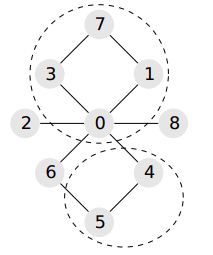
\includegraphics{1.png}

Возможным корректным решением является $[1, 1, 3, 1, 2, 2, 3, 1, 3]$., которое
соответствует следующему разбиению: $A=\{0, 1, 3, 7\}$, $B=\{4, 5\}$, $C=\{2, 6, 8\}$.
Множества $A$ и $B$ являются связными.

\textbf{Пример 2}

Рассмотрим следующий вызов:

\texttt{find\_split(6, 2, 2, 2, [0, 0, 0, 0, 0], [1, 2, 3, 4, 5])}

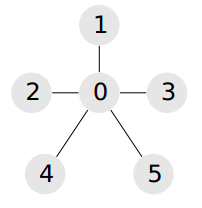
\includegraphics{2.png}

Корректного разбиения не существует, поэтому единственным верным ответом является $[0, 0, 0, 0, 0, 0]$.
